% ============================================================================
% Deliverable 3 - Generative Artificial Intelligence (580694), Primavera 2026
% Documento tecnico: UNA pagina vertical.
%
% Las cifras NO se escriben a mano: salen de results_d3/ via
%     python -m d3.report results_d3 && python report/fill_d3.py results_d3
% que genera report/d3_numbers.tex. Compilar:  pdflatex deliverable3_es.tex (x2)
% ============================================================================
\newcommand{\EQUIPO}{Pedro Dañobeytia \textbullet\ Rafael Fernández \textbullet\ Cristian González \textbullet\ Daniel González}
\newcommand{\REPO}{github.com/Rafaefe/AIBattlesInPokemon}
\newcommand{\VIDEO}{\ph{link del video}}

\documentclass[9pt,a4paper]{extarticle}
\usepackage[utf8]{inputenc}
\usepackage[T1]{fontenc}
\usepackage[margin=0.7cm,top=0.5cm,bottom=0.4cm]{geometry}
\usepackage{helvet}\renewcommand{\familydefault}{\sfdefault}
\usepackage{xcolor}
\usepackage{booktabs}
\usepackage{enumitem}
\usepackage{multicol}
\usepackage{tcolorbox}
\usepackage{tikz}
\usepackage{microtype}
\usetikzlibrary{arrows.meta,positioning}

\hyphenpenalty=10000 \exhyphenpenalty=10000 \tolerance=3000 \emergencystretch=2.5em

\definecolor{navy}{HTML}{16314F}
\definecolor{steel}{HTML}{3C5A80}
\definecolor{amber}{HTML}{B45309}
\definecolor{crimson}{HTML}{9B1C1C}
\definecolor{teal}{HTML}{0F766E}
\definecolor{rule}{HTML}{C9D2DE}
\definecolor{note}{HTML}{FDF3D8}
\definecolor{mint}{HTML}{E6F4F1}
\definecolor{lav}{HTML}{EFEAF7}
\definecolor{plum}{HTML}{6B3FA0}

\setlength{\parindent}{0pt}
\setlength{\parskip}{0.4mm}
\setlength{\columnsep}{5mm}
\setlength{\multicolsep}{1pt}
\setlength{\tabcolsep}{3pt}
\pagestyle{empty}

\newcommand{\ph}[1]{\colorbox{yellow!60}{\textcolor{black}{\textbf{#1}}}}
% GENERADO por report/fill_d3.py -- no editar a mano.
\newcommand{\accBaseA}{\ph{??}}
\newcommand{\accBaseH}{\ph{??}}
\newcommand{\accBaseO}{\ph{??}}
\newcommand{\accFullA}{\ph{??}}
\newcommand{\accFullH}{\ph{??}}
\newcommand{\accFullO}{\ph{??}}
\newcommand{\accHeurA}{\ph{??}}
\newcommand{\accHeurH}{\ph{??}}
\newcommand{\accHeurO}{\ph{??}}
\newcommand{\accNoDecA}{\ph{??}}
\newcommand{\accNoDecH}{\ph{??}}
\newcommand{\accNoDecO}{\ph{??}}
\newcommand{\accNoFewA}{\ph{??}}
\newcommand{\accNoFewH}{\ph{??}}
\newcommand{\accNoFewO}{\ph{??}}
\newcommand{\accNoRagA}{\ph{??}}
\newcommand{\accNoRagH}{\ph{??}}
\newcommand{\accNoRagO}{\ph{??}}
\newcommand{\accNoRankA}{\ph{??}}
\newcommand{\accNoRankH}{\ph{??}}
\newcommand{\accNoRankO}{\ph{??}}
\newcommand{\accNoVerA}{\ph{??}}
\newcommand{\accNoVerH}{\ph{??}}
\newcommand{\accNoVerO}{\ph{??}}
\newcommand{\accStwoA}{\ph{??}}
\newcommand{\accStwoH}{\ph{??}}
\newcommand{\accStwoO}{\ph{??}}
\newcommand{\alwaysOne}{\ph{??}}
\newcommand{\callsBase}{\ph{??}}
\newcommand{\callsFull}{\ph{??}}
\newcommand{\callsHeur}{\ph{??}}
\newcommand{\callsNoDec}{\ph{??}}
\newcommand{\callsNoFew}{\ph{??}}
\newcommand{\callsNoRag}{\ph{??}}
\newcommand{\callsNoRank}{\ph{??}}
\newcommand{\callsNoVer}{\ph{??}}
\newcommand{\callsStwo}{\ph{??}}
\newcommand{\chiPBase}{\ph{??}}
\newcommand{\chiPFull}{\ph{??}}
\newcommand{\chiPHeur}{\ph{??}}
\newcommand{\chiPNoDec}{\ph{??}}
\newcommand{\chiPNoFew}{\ph{??}}
\newcommand{\chiPNoRag}{\ph{??}}
\newcommand{\chiPNoRank}{\ph{??}}
\newcommand{\chiPNoVer}{\ph{??}}
\newcommand{\chiPStwo}{\ph{??}}
\newcommand{\ciBaseA}{\ph{??}}
\newcommand{\ciBaseH}{\ph{??}}
\newcommand{\ciBaseO}{\ph{??}}
\newcommand{\ciFullA}{\ph{??}}
\newcommand{\ciFullH}{\ph{??}}
\newcommand{\ciFullO}{\ph{??}}
\newcommand{\ciHeurA}{\ph{??}}
\newcommand{\ciHeurH}{\ph{??}}
\newcommand{\ciHeurO}{\ph{??}}
\newcommand{\ciNoDecA}{\ph{??}}
\newcommand{\ciNoDecH}{\ph{??}}
\newcommand{\ciNoDecO}{\ph{??}}
\newcommand{\ciNoFewA}{\ph{??}}
\newcommand{\ciNoFewH}{\ph{??}}
\newcommand{\ciNoFewO}{\ph{??}}
\newcommand{\ciNoRagA}{\ph{??}}
\newcommand{\ciNoRagH}{\ph{??}}
\newcommand{\ciNoRagO}{\ph{??}}
\newcommand{\ciNoRankA}{\ph{??}}
\newcommand{\ciNoRankH}{\ph{??}}
\newcommand{\ciNoRankO}{\ph{??}}
\newcommand{\ciNoVerA}{\ph{??}}
\newcommand{\ciNoVerH}{\ph{??}}
\newcommand{\ciNoVerO}{\ph{??}}
\newcommand{\ciStwoA}{\ph{??}}
\newcommand{\ciStwoH}{\ph{??}}
\newcommand{\ciStwoO}{\ph{??}}
\newcommand{\dropBase}{\ph{??}}
\newcommand{\dropFull}{\ph{??}}
\newcommand{\dropHeur}{\ph{??}}
\newcommand{\dropNoDec}{\ph{??}}
\newcommand{\dropNoFew}{\ph{??}}
\newcommand{\dropNoRag}{\ph{??}}
\newcommand{\dropNoRank}{\ph{??}}
\newcommand{\dropNoVer}{\ph{??}}
\newcommand{\dropStwo}{\ph{??}}
\newcommand{\factsRight}{\ph{??}}
\newcommand{\factsRightNoFew}{\ph{??}}
\newcommand{\factsRightNoRag}{\ph{??}}
\newcommand{\failCauses}{\ph{??}}
\newcommand{\fcCause}{\ph{??}}
\newcommand{\fcChosen}{\ph{??}}
\newcommand{\fcDiff}{\ph{??}}
\newcommand{\fcFacts}{\ph{??}}
\newcommand{\fcId}{\ph{??}}
\newcommand{\fcRef}{\ph{??}}
\newcommand{\fcRegret}{\ph{??}}
\newcommand{\gainBase}{\ph{??}}
\newcommand{\gainFull}{\ph{??}}
\newcommand{\gainHeur}{\ph{??}}
\newcommand{\gainNoDec}{\ph{??}}
\newcommand{\gainNoFew}{\ph{??}}
\newcommand{\gainNoRag}{\ph{??}}
\newcommand{\gainNoRank}{\ph{??}}
\newcommand{\gainNoVer}{\ph{??}}
\newcommand{\gainStwo}{\ph{??}}
\newcommand{\hw}{\ph{??}}
\newcommand{\libs}{\ph{??}}
\newcommand{\lookupPct}{\ph{??}}
\newcommand{\loopBroken}{\ph{??}}
\newcommand{\loopFixed}{\ph{??}}
\newcommand{\lossBase}{\ph{??}}
\newcommand{\lossFull}{\ph{??}}
\newcommand{\lossHeur}{\ph{??}}
\newcommand{\lossNoDec}{\ph{??}}
\newcommand{\lossNoFew}{\ph{??}}
\newcommand{\lossNoRag}{\ph{??}}
\newcommand{\lossNoRank}{\ph{??}}
\newcommand{\lossNoVer}{\ph{??}}
\newcommand{\lossStwo}{\ph{??}}
\newcommand{\modelId}{\ph{??}}
\newcommand{\modelRev}{\ph{??}}
\newcommand{\nAll}{\ph{??}}
\newcommand{\nDeviated}{\ph{??}}
\newcommand{\nFacts}{\ph{??}}
\newcommand{\nFail}{\ph{??}}
\newcommand{\nParams}{\ph{??}}
\newcommand{\nPlanMissed}{\ph{??}}
\newcommand{\nRevised}{\ph{??}}
\newcommand{\nUnverified}{\ph{??}}
\newcommand{\pBase}{\ph{??}}
\newcommand{\pFull}{\ph{??}}
\newcommand{\pFullBase}{\ph{??}}
\newcommand{\pFullFull}{\ph{??}}
\newcommand{\pFullHeur}{\ph{??}}
\newcommand{\pFullNoDec}{\ph{??}}
\newcommand{\pFullNoFew}{\ph{??}}
\newcommand{\pFullNoRag}{\ph{??}}
\newcommand{\pFullNoRank}{\ph{??}}
\newcommand{\pFullNoVer}{\ph{??}}
\newcommand{\pFullStwo}{\ph{??}}
\newcommand{\pHeur}{\ph{??}}
\newcommand{\pNoDec}{\ph{??}}
\newcommand{\pNoFew}{\ph{??}}
\newcommand{\pNoRag}{\ph{??}}
\newcommand{\pNoRank}{\ph{??}}
\newcommand{\pNoVer}{\ph{??}}
\newcommand{\pStwo}{\ph{??}}
\newcommand{\rightSection}{\ph{??}}
\newcommand{\winBase}{\ph{??}}
\newcommand{\winFull}{\ph{??}}
\newcommand{\winHeur}{\ph{??}}
\newcommand{\winNoDec}{\ph{??}}
\newcommand{\winNoFew}{\ph{??}}
\newcommand{\winNoRag}{\ph{??}}
\newcommand{\winNoRank}{\ph{??}}
\newcommand{\winNoVer}{\ph{??}}
\newcommand{\winStwo}{\ph{??}}


\newcommand{\heading}[1]{%
  \par\vspace{0.8mm}\noindent
  {\color{navy}\bfseries\MakeUppercase{#1}}\par\vspace{0.2mm}
  {\color{amber}\hrule height 0.8pt}\vspace{0.6mm}\noindent\ignorespaces}
\newtcolorbox{keybox}[1]{colback=note,colframe=amber,boxrule=0.6pt,left=1.2mm,right=1.2mm,top=0.6mm,bottom=0.6mm,arc=1mm,
  before skip=1mm,after skip=0.6mm,fonttitle=\bfseries,coltitle=white,colbacktitle=amber,title={#1}}
\newtcolorbox{failbox}[1]{colback=white,colframe=crimson,boxrule=0.6pt,left=1.2mm,right=1.2mm,top=0.6mm,bottom=0.6mm,arc=1mm,
  before skip=1mm,after skip=0.6mm,fonttitle=\bfseries,coltitle=white,colbacktitle=crimson,title={#1}}
\setlist[itemize]{leftmargin=3mm,itemsep=0.2mm,topsep=0.3mm,parsep=0pt}

\begin{document}
\small

% ================================================================ CABECERA ==
\begin{tcolorbox}[colback=navy,colframe=navy,boxrule=0pt,left=2.5mm,right=2.5mm,top=1.2mm,bottom=1.2mm,arc=1mm,after skip=1mm]
{\color{white}\bfseries\large Consultar en vez de recordar: tres agentes de 1{,}5B juegan Pok\'emon Blue}\hfill
{\color{white!80}\footnotesize Deliverable 3 \textbullet\ GenAI (580694) \textbullet\ UdeC}\\[0.6mm]
{\footnotesize\color{white!85}Equipo:} {\footnotesize\bfseries\color{white}\EQUIPO}\hfill
{\footnotesize\color{white!85}Repo:} {\footnotesize\color{white}\texttt{\REPO}} \quad
{\footnotesize\color{white!85}Video:} {\footnotesize\color{white}\VIDEO}
\end{tcolorbox}

% ================================================================== GRAFO ==
{\centering
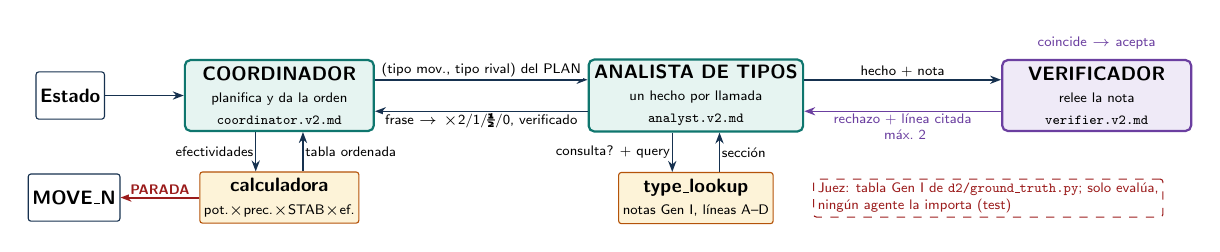
\begin{tikzpicture}[font=\scriptsize,
  agent/.style={draw=teal,fill=mint,line width=0.8pt,rounded corners=2pt,align=center,inner sep=2pt,minimum height=9mm,minimum width=24mm},
  ver/.style={agent,draw=plum,fill=lav},
  tool/.style={draw=amber,fill=note,rounded corners=1pt,align=center,inner sep=1.5pt,minimum height=6.5mm},
  io/.style={draw=navy,fill=white,rounded corners=1pt,align=center,inner sep=1.5pt,minimum height=6mm,font=\scriptsize\bfseries},
  arr/.style={-{Stealth[length=1.4mm]},line width=0.55pt,draw=navy},
  lbl/.style={font=\tiny,fill=white,inner sep=0.6pt,align=center}]
\node[io] (env) {Estado};
\node[agent,right=10mm of env] (co) {\textbf{COORDINADOR}\\{\tiny planifica y da la orden}\\{\tiny\texttt{coordinator.v2.md}}};
\node[agent,right=27mm of co] (an) {\textbf{ANALISTA DE TIPOS}\\{\tiny un hecho por llamada}\\{\tiny\texttt{analyst.v2.md}}};
\node[ver,right=25mm of an] (ve) {\textbf{VERIFICADOR}\\{\tiny relee la nota}\\{\tiny\texttt{verifier.v2.md}}};
\node[tool,below=5mm of an] (kb) {\textbf{type\_lookup}\\{\tiny notas Gen I, l\'ineas A--D}};
\node[tool,below=5mm of co] (calc) {\textbf{calculadora}\\{\tiny pot.$\times$prec.$\times$STAB$\times$ef.}};
\node[io,left=10mm of calc] (out) {MOVE\_N};
\draw[arr] (env) -- (co);
\draw[arr] ([yshift=2mm]co.east) -- node[lbl,above]{(tipo mov., tipo rival) del PLAN} ([yshift=2mm]an.west);
\draw[arr] ([yshift=-2mm]an.west) -- node[lbl,below]{frase $\to\times$2/1/\textonehalf/0, verificado} ([yshift=-2mm]co.east);
\draw[arr] ([yshift=2mm]an.east) -- node[lbl,above]{hecho + nota} ([yshift=2mm]ve.west);
\draw[arr,draw=plum] ([yshift=-2mm]ve.west) -- node[lbl,below,text=plum]{rechazo + l\'inea citada\\$\circlearrowleft$ m\'ax.\ 2} ([yshift=-2mm]an.east);
\draw[arr] ([xshift=-3mm]an.south) -- node[lbl,left]{consulta? + query} ([xshift=-3mm]kb.north);
\draw[arr] ([xshift=3mm]kb.north) -- node[lbl,right]{secci\'on} ([xshift=3mm]an.south);
\draw[arr] ([xshift=-3mm]co.south) -- node[lbl,left]{efectividades} ([xshift=-3mm]calc.north);
\draw[arr] ([xshift=3mm]calc.north) -- node[lbl,right]{tabla ordenada} ([xshift=3mm]co.south);
\draw[arr,draw=crimson,line width=0.7pt] (calc.west) -- node[lbl,above,text=crimson]{\textbf{PARADA}} (out.east);
\node[font=\tiny,text=plum,above=0mm of ve.north] {coincide $\to$ acepta};
\node[draw=crimson,dashed,rounded corners=1pt,font=\tiny,text=crimson,right=5mm of kb,align=left,inner sep=1.5pt]
  {Juez: tabla Gen I de \texttt{d2/ground\_truth.py}; solo eval\'ua,\\ning\'un agente la importa (test)};
\end{tikzpicture}\par}
{\centering\scriptsize Los tres agentes usan el \textbf{mismo} \texttt{\modelId} (\nParams\,B), greedy, \hw\ (\libs). Verde/lila = agentes (llamadas al modelo); \'ambar = herramientas.\par}

\begin{multicols}{2}
% ============================================================ 1. CONTINUIDAD
\heading{1. Continuidad con D1 y D2}
\textbf{Misma tarea y criterio:} estado $\to$ \texttt{MOVE\_N}; correcto = m\'aximo de potencia$\times$precisi\'on$\times$STAB$\times$efectividad Gen I, sobre los \textbf{mismos \nAll\ estados} del D2 (semillas 20260830 y 20260927). \textbf{Mismo fallo, en su forma del D2:} sin sesgo de posici\'on, pero el modelo \emph{no sabe} la tabla (``normal damage'' en el 87\,\% de los pares). \textbf{Desviaci\'on declarada:} ahora el Analista \emph{consulta} un texto con la tabla (\texttt{d3/kb/}), separado del juez y verificado contra \'el en los 196 pares por un test. La D3 mide si el modelo sabe \emph{usar} la tabla, no si la recuerda.

% ============================================================ 2. AGENTES
\heading{2. Agentes}
{\scriptsize
\begin{tabular}{@{}p{0.16\linewidth}p{0.37\linewidth}p{0.41\linewidth}@{}}
\toprule
\textbf{Agente} & \textbf{Recibe $\to$ devuelve} & \textbf{Decide / se detiene}\\
\midrule
Coordinador & estado $\to$ \texttt{PLAN}; tabla $\to$ \texttt{MOVE\_N} & qu\'e movimientos se analizan; \textbf{para} al emitir \texttt{MOVE\_N}\\
Analista & (atacante, defensor[, rechazo]) $\to$ frase del juego & si consulta y qu\'e; lee la nota l\'inea por l\'inea\\
Verificador & hecho + nota $\to$ l\'inea A--D & acepta si coincide; si no, lo devuelve citando la l\'inea (m\'ax.\ 2)\\
\bottomrule
\end{tabular}}

\textbf{Por qu\'e tres:} \emph{saber} el hecho (fallo del D2) es del Analista con la herramienta; \emph{comprobarlo} lo hace otro agente que no lo produjo; \emph{combinar} las 4 opciones (fallo del D1) queda en la calculadora, y el Coordinador decide sobre la tabla ya ordenada. Prompts versionados en \texttt{d3/prompts/} (sha256 en cada traza); las v2 se ajustaron antes de evaluar con sondeos del modelo real.

% ============================================================ 3. TECNICAS
\heading{3. T\'ecnicas y su contribuci\'on (\nAll\ estados)}
{\scriptsize
\begin{tabular}{@{}llp{0.25\linewidth}rr@{}}
\toprule
\textbf{Agente} & \textbf{T\'ecnica} & \textbf{Contra} & \textbf{sin ella} & \textbf{compl.\ +/--}\\
\midrule
Analista & recuperaci\'on (ReAct+RAG) & no sabe la tabla & \accNoRagA\,\% & +\gainNoRag/--\dropNoRag\\
Coordinador & descomposici\'on & combinar 4 opciones & \accNoDecA\,\% & +\gainNoDec/--\dropNoDec\\
Coordinador & tabla ordenada & sesgo de posici\'on & \accNoRankA\,\% & +\gainNoRank/--\dropNoRank\\
Verificador & verificaci\'on + bucle & leer mal la nota & \accNoVerA\,\% & +\gainNoVer/--\dropNoVer\\
Verificador & few-shot (3 ejemplos) & revisar mal & \accNoFewA\,\% & +\gainNoFew/--\dropNoFew\\
\bottomrule
\end{tabular}}
{\scriptsize ``Sin ella'': el sistema completo (\accFullA\,\%) con \emph{solo} esa t\'ecnica apagada. +/--: estados que el completo gana/pierde frente a la ablaci\'on (McNemar: recuperaci\'on $p{=}\pFullNoRag$, orden $p{=}\pFullNoRank$, few-shot $p{=}\pFullNoFew$). Todos usan rol en el \emph{system prompt} y salida restringida.}

\textbf{El few-shot resta: contamina.} Los ejemplos del Verificador nombran tipos (``List: Water-type, Flying-type \ldots\ yes'') y el modelo copia esas respuestas: \nWrongWater\ de los \nWrongFull\ hechos err\'oneos tienen defensor Water (Normal$\to$Water ``super effective''). Sin few-shot hay \nWrongNoFew\ hechos err\'oneos; con \'el, el bucle corrige \loopFixed\ y da\~na \loopBroken.

% ============================================================ RESULTADO
\begin{keybox}{Resultado en breve}
B0 \accBaseA\,\% $\to$ S2 \accStwoA\,\% $\to$ \textbf{agentes \accFullA\,\%}. Gana/pierde frente a B0 \winFull/\lossFull\ ($p{=}\pFull$), frente a S2 \gainStwo/\dropStwo\ ($p{=}\pFullStwo$) y, por primera vez, frente a H (ignora tipos, \accHeurA\,\%) \gainHeur/\dropHeur\ ($p{=}\pFullHeur$). Hechos de tipos correctos: \factsRightNoRag\,\% de memoria $\to$ \textbf{\factsRight\,\%} consultando.
\end{keybox}

% ============================================================ 4. RESULTADOS
\heading{4. Evidencia: mismos estados, mismo criterio}
{\centering\scriptsize
\begin{tabular}{@{}lrrrr@{}}
\toprule
& \textbf{50 orig.} & \textbf{50 nuevos} & \textbf{\nAll\ [IC 95\%]} & \textbf{llam.}\\
\midrule
B0 directo (baseline) & \accBaseO\,\% & \accBaseH\,\% & \accBaseA\,\% [\ciBaseA] & \callsBase\\
H sin modelo & \accHeurO\,\% & \accHeurH\,\% & \accHeurA\,\% [\ciHeurA] & 0\\
S2 soluci\'on D2 & \accStwoO\,\% & \accStwoH\,\% & \accStwoA\,\% [\ciStwoA] & \callsStwo\\
\textbf{D3 completo} & \textbf{\accFullO\,\%} & \textbf{\accFullH\,\%} & \textbf{\accFullA\,\%} [\ciFullA] & \callsFull\\
\midrule
\quad sin recuperaci\'on & \accNoRagO\,\% & \accNoRagH\,\% & \accNoRagA\,\% [\ciNoRagA] & \callsNoRag\\
\quad sin descomposici\'on & \accNoDecO\,\% & \accNoDecH\,\% & \accNoDecA\,\% [\ciNoDecA] & \callsNoDec\\
\quad sin tabla ordenada & \accNoRankO\,\% & \accNoRankH\,\% & \accNoRankA\,\% [\ciNoRankA] & \callsNoRank\\
\quad sin Verificador & \accNoVerO\,\% & \accNoVerH\,\% & \accNoVerA\,\% [\ciNoVerA] & \callsNoVer\\
\quad sin few-shot & \accNoFewO\,\% & \accNoFewH\,\% & \accNoFewA\,\% [\ciNoFewA] & \callsNoFew\\
\bottomrule
\end{tabular}\par}

% ============================================================ 5. FALLO
\begin{failbox}{5. Caso de fallo: estado \fcId\ (\fcDiff)}
\footnotesize Rival Poison/Psychic. Eligi\'o \fcChosen\ (Psychic); el \'optimo era \fcRef\ (Blizzard): pierde el \fcRegret\,\% del score. \textbf{Por qu\'e} (\texttt{traces/demo\_holdout48\_full.json}): la nota dice ``B. Not very effective against: Psychic-type''. El Verificador, con ejemplos donde 2 de 3 respuestas son ``no'', le dio P(yes)$\,{=}\,$0{,}20, concluy\'o ``l\'inea D'' y devolvi\'o el hecho; el Analista acept\'o ``normal damage'' (Gen I: $\times$0{,}5). Psychic qued\'o con 180 en vez de 90 y super\'o a Blizzard (108). \textbf{El revisor introdujo el error.} Fallos del completo: \nFail\ (\failCauses).
\end{failbox}

% ============================================================ 6. LIMITES
\heading{6. L\'imites}
\begin{itemize}
\item \textbf{Revisor y revisado son el mismo modelo:} cuando el Verificador lee mal, el bucle propaga su error.
\item \textbf{El mejor medido no es el reportado:} sin few-shot se llega a \accNoFewA\,\%, pero sale de los mismos estados que revelaron el problema (y las v2 se ajustaron con pares de ellos): falta confirmarlo en estados nuevos.
\item \textbf{Coordinador:} plan incompleto en \nPlanMissed\ estados; se apart\'o del m\'aximo de la calculadora en \nDeviated.
\item \textbf{Costo:} \callsFull\ llamadas por estado (B0: 1; S2: \callsStwo). Como en D1 y D2, solo da\~no inmediato.
\end{itemize}
\end{multicols}

\vspace{-1mm}
{\centering\scriptsize\color{black!70}Reproducir: \texttt{python -m d3.evaluate} \textbullet\ \texttt{python -m d3.demo [--seed N | --replay orig:ID]} \textbullet\ trazas: \texttt{results\_d3/*/traces/}, \texttt{traces/} \textbullet\ cifras: \texttt{python report/fill\_d3.py}\par}
\end{document}
